\subsubsection{\textit{Bubbling}}

\paragraph{Lema \ref{lemma:bcount}: \texttt{bubbling\_counts\_n}:} seja $l$ uma lista de números naturais, e lembrando
que \texttt{bubbling\_count} é uma função que retorna um par $(l,c)$, onde $c$ denota o número
de comparações realizadas ao todo na chamada
\begin{equation*}
    \forall_{l,n,c} bubbling\_count(l, c, n)_2 = c + n \hspace{1cm}, n<|l|, c\in \mathbb{N}
\end{equation*}

\paragraph{Estratégia da prova:} indução forte sobre $|l|$.
A função \texttt{bubbling\_count} faz chamadas recursivas sobre $l$, e seria
correspondente às linhas 5 a 9 do Algoritmo \ref{algo:bubblesort}.
Cada chamada é feita sobre uma lista menor mas a lista não é dividida
exatamente conforme a definição recursiva de $l$. Portanto precisamos de
uma medida alternativa que seja relacionada com a estrutura
sobre a qual queremos realizar a indução (Figura \ref{fig:bubbling1}).

\begin{figure}[h!]
    \centering
    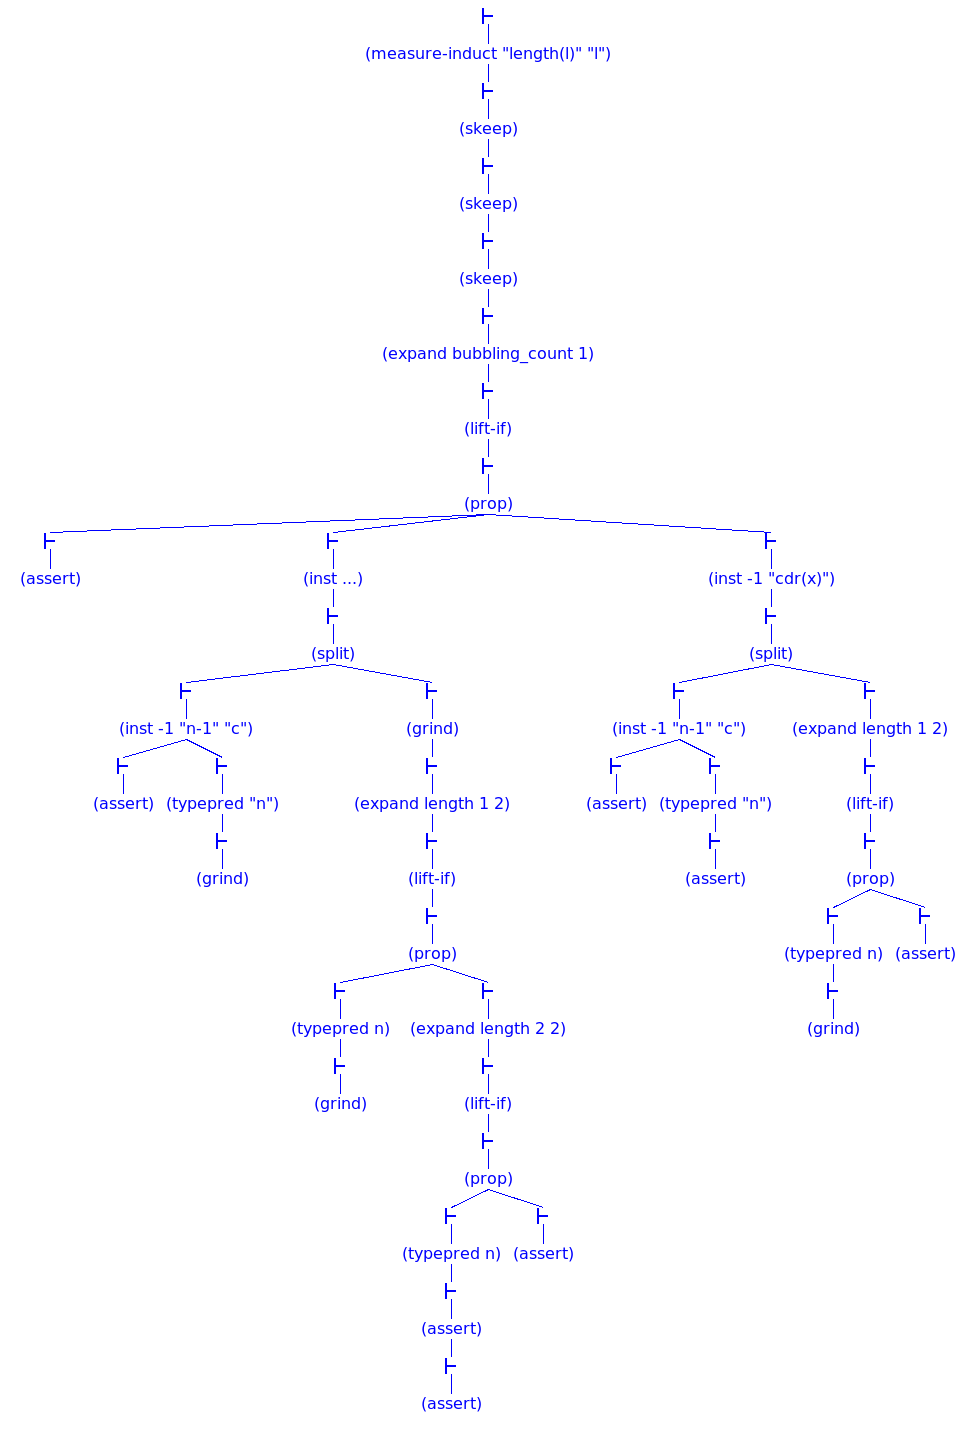
\includegraphics[width=0.5\linewidth,trim={8cm 35cm 8cm 0},clip]{figures/bubbling-counts-n.png}
    \caption{A prova do lema de complexidade de \texttt{bubbling\_count} foi realizada
    por indução forte sobre $|l|$.}
    \label{fig:bubbling1}
\end{figure}

Após a expansão da definição da definição de \texttt{bubbling\_count}, precisamos
provar 3 casos: o caso em que $n=0$ (trivial, pois $c = c + n = c + 0 = c$), 
o caso em que $l_i > l_{i+1}$ e o caso em que $l_i \leq l_{i+1}$. A prova destes dois
últimos casos é muito semelhante, e varia essencialmente em como a hipótese de indução
(\HI) será instanciada (Figura \ref{fig:bubbling2}). No primeiro caso,
a próxima chamada de \texttt{bubbling\_count} será realizada sobre uma lista com a
forma $l_i:l_{i+2}:l'_{i+2}$, portanto essa deve ser a instanciação da \HI.

\begin{lstlisting}
{-1}  car(x) > car(cdr(x))
[-2]  (H.I.)
  |-------
{1}   1 + bubbling_count(cons(car(x), cdr(cdr(x))), c, n - 1)`2 = c + n
{2}   n = 0

Rule? (inst -2 "cons(car(x), cdr(cdr(x)))")
\end{lstlisting} 

No segundo caso, a próxima chamada \texttt{bubbling\_count} será propriamente sobre
a cauda de $l_i$, portanto a \HI é instanciada como $l'_i$:

\begin{lstlisting}
[-1]  (H.I.)
  |-------
{1}   car(x) > car(cdr(x))
{2}   1 + bubbling_count(cdr(x), c, n - 1)`2 = c + n
{3}   n = 0

Rule? (inst -1 "cdr(x)")
\end{lstlisting} 

\begin{figure}[h!]
    \centering
    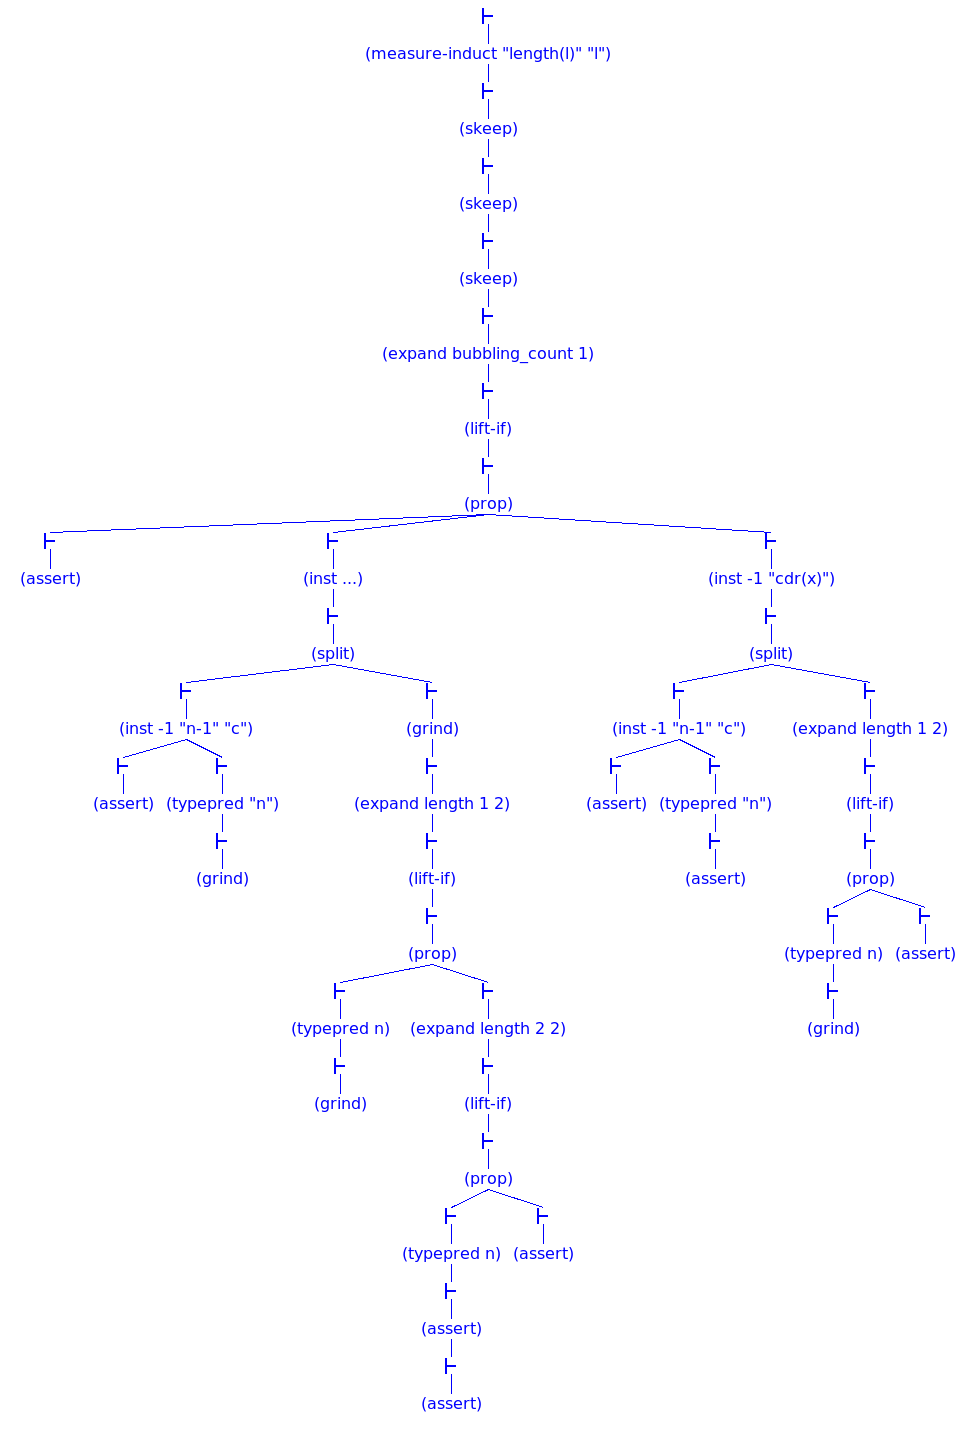
\includegraphics[width=0.75\linewidth,trim={8cm 20cm 4cm 10cm},clip]{figures/bubbling-counts-n.png}
    \caption{Casos da prova após a expansão da definição de \texttt{bubbling\_count}. O
    ramo omitido mais à esquerda é o caso base.}
    \label{fig:bubbling2}
\end{figure}


O restante da prova consiste em algumas instanciações adicionais de $c$ e/ou $n$, 
na expansão da definição de \texttt{length} e inferências sobre o tipo de $n$.
Felizmente existe a restrição de que $n < |l|$, e o comando \texttt{(typepred n)}
realiza essa inferência. O uso de \texttt{(grind)} após \texttt{(typepred n)}
foi basicamente um atalho para \texttt{(expand list2finseq)}
seguido de \texttt{(assert)}, ou de alguma resolução dos casos distintos
de \texttt{length}, que surge a partir da definição de \texttt{list2finseq}
(Figura \ref{fig:bubbling3}).

\begin{figure}[h!]
    \centering
    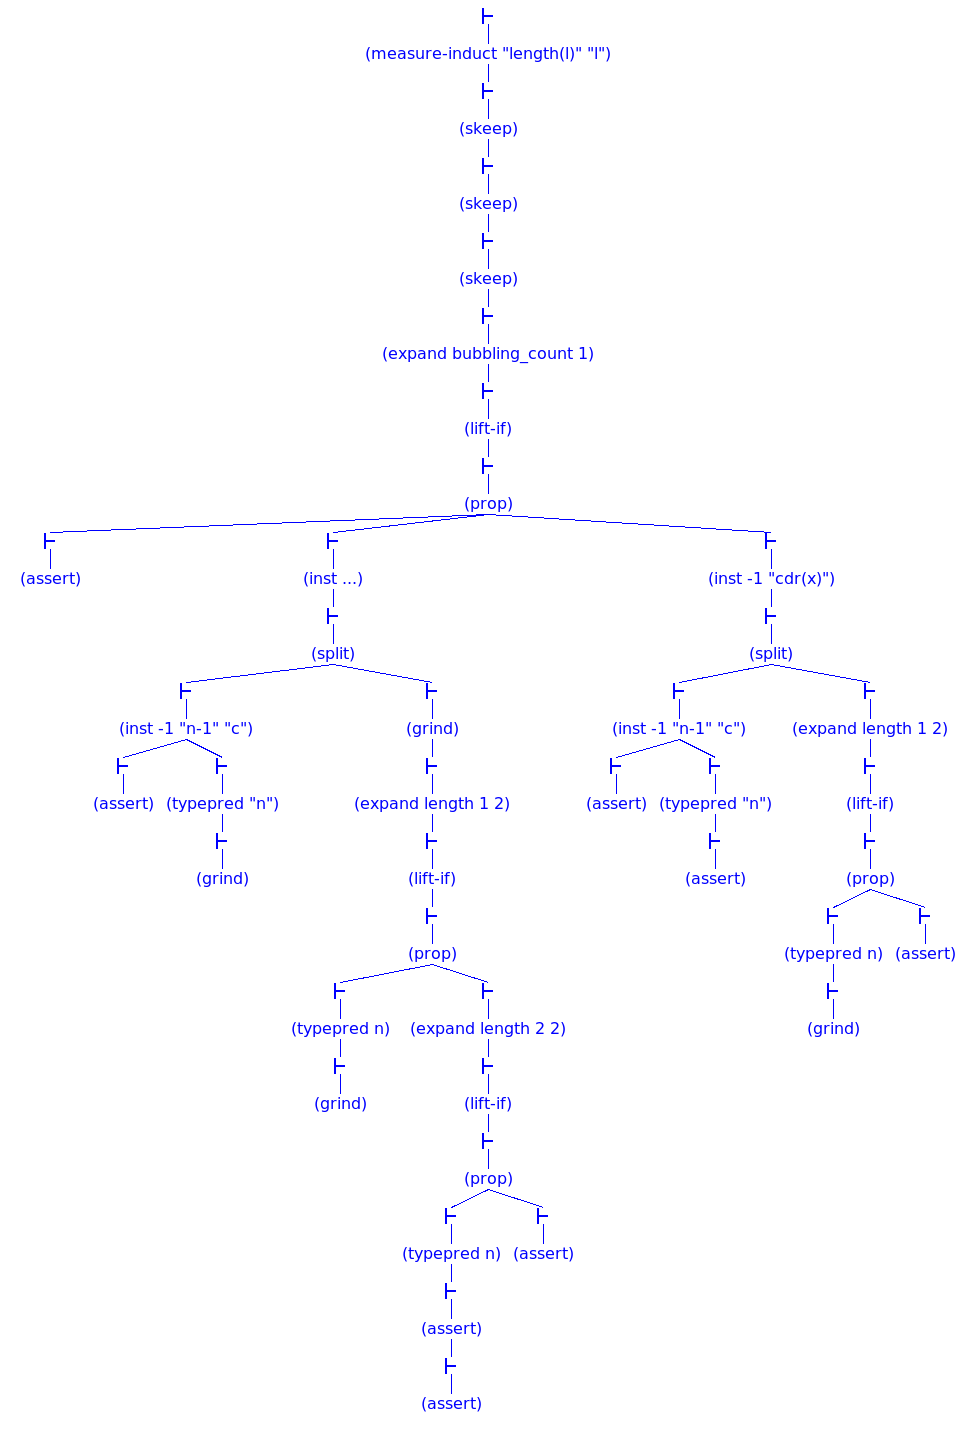
\includegraphics[width=0.25\linewidth,trim={20.5cm 10cm 0cm 18.5cm},clip]{figures/bubbling-counts-n.png}
    \caption{Para finalizar os ramos, foi necessário expandir a definição de
    \texttt{length} e realizar uma inferência sobre o tipo de $n$.}
    \label{fig:bubbling3}
\end{figure}


Dizemos então que \texttt{bubbling\_count} tem complexidade linear, $O(n)$.
Como $n<|l|$ por definição, então a função também é $O(|l|)$.
Resta então mostrar que o mesmo
se aplica a função original, \texttt{bubbling}, e isto foi feito mostrando que
\texttt{bubbling} e \texttt{bubbling\_count} são equivalentes:

\paragraph{Lema \ref{lemma:bequiv}: \texttt{bubbling\_equiv}:} 
\begin{equation*}
    \forall_{l,n,c} bubbling(l, n)_1 = bubbling\_count(l, c, n)_1 \hspace{1cm}, n<|l|, c\in \mathbb{N}
\end{equation*}

\paragraph{Estratégia da prova:} indução forte sobre $|l|$, pelo mesmo motivo
que no lema \ref{lemma:bcount} já que a prova se refere à mesma função,
\texttt{bubbling\_count}, que divide a lista da mesma forma que
\texttt{bubbling}. A diferença principal entre prova deste lema e a do lema
\ref{lemma:bcount} é que é necessário expandir as definições de ambas as
funções, \texttt{bubbling} e \texttt{bubbling\_count} antes de instanciar
a \HI. As instanciações da \HI foram realizdas como na prova do
lema \ref{lemma:bcount} (Figura \ref{fig:bubbling4}).

\begin{figure}[H]
    \centering
    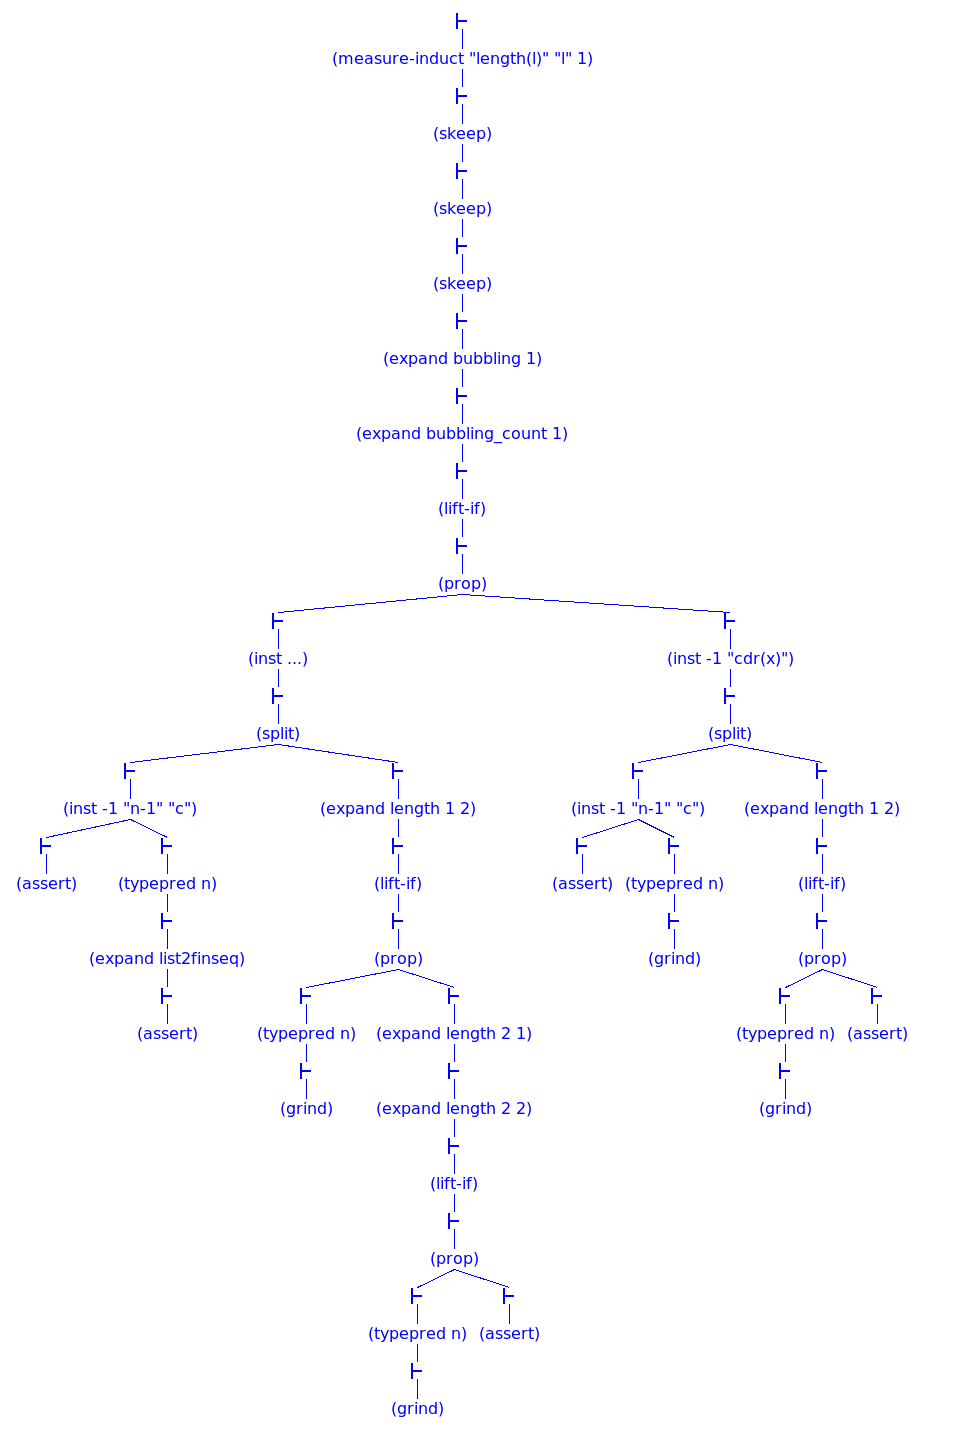
\includegraphics[width=0.\linewidth,trim={5cm 19cm 3cm 8cm},clip]{figures/bubbling-equiv.png}
    \caption{A prova do lema de equivalência entre \texttt{bubbling} e
    \texttt{bubbling\_count} requer a expansão de ambas as funções,
    mas segue de forma semelhante ao lema de complexidade.}
    \label{fig:bubbling4}
\end{figure}


\paragraph{Lema \ref{lemma:blen}: \texttt{bubbling\_length}:}
\begin{equation*}
    \forall_{l,n,c} |bubbling\_count(l, c, n)_1| = |l| \hspace{1cm}, n<|l|, c\in \mathbb{N}
\end{equation*}

\paragraph{Estratégia da prova:} indução forte sobre $|l|$, pelo mesmo motivo
que no lema \ref{lemma:bcount} já que a prova se refere à mesma função,
\texttt{bubbling\_count}. Este lema não está diretamente relacionado com
a analise da complexidade ou com a equivalência entre as funções. Contudo,
ele foi utilizado em alguns pontos das provas subsequentes e, por se tratar
de um lema relativamente longo de ser provado, decidimos enunciá-lo
separadamente. O objetivo deste lema é mostrar que \texttt{bubbling\_count}
retorna uma lista do mesmo tamanho que a lista de entrada, e a prova também
consiste em mostrar que isso é verdade para cada um dos casos da função
\texttt{bubbling\_count}.


